\subsection*{Показатель Хёрста}
\addcontentsline{toc}{subsection}{Показатель Хёрста}

\textbf{Задание:}\\
Рассчитать показатель Хёрста для проверки рядов на наличие персистентности.\\

\textbf{Решение:}\\
Существуют различные способы определения фрактальных размерностей, к числу которых относится R/S метод, на основании которого определяется показатель Хёрста. Этот показатель имеет широкое применени в анализе временных рядов благодаря своей устойчивости. Он содержит минимальные предположения об изучаемой системе и может классифицировать временные ряды, позволяет отличить случайный ряд от неслучайного, даже если случайный ряд не является нормально распределенным.\\

Пусть имеется некоторый временной ряд $X$. Пусть $S$ -- среднеквадратическое отклонение ряда, $N$ -- количество наблюдений, $R$ -- максимальный размах ряда.\\

Для вычисления размаха $R$ можно применить следующий алгоритм:\\
\begin{enumerate}[topsep=0pt,itemsep=-1ex,partopsep=1ex,parsep=1ex]
	\item вычислить среднее значение ряда ($\bar{x}$) и среднеквадратическое отклонение $S$;
	\item получить ряд: $y_1 = x_1 - \bar{x}$, $y_2 = x_1 + x_2 - 2 \bar{x}$, \dots, $y_N = x_1 + x_2 + \dots + x_N - N \bar{x}$;
	\item вычислить: $R = \max Y - \min Y$.\\
\end{enumerate}

Когда будет вычислено значение размаха, то можно воспользоваться формулой, для нахождения показателя Хёрста:

\[ H = \dfrac{\ln \dfrac{R}{S}}{\ln a N} \]

\newpage

В соответствии с рассмотренными алгоритмами, для вычисления показателя Хёрста была написана функция на языке программирования Python. (Рисунок \ref{fig:hearst1})
\begin{figure}[h]
	\centering 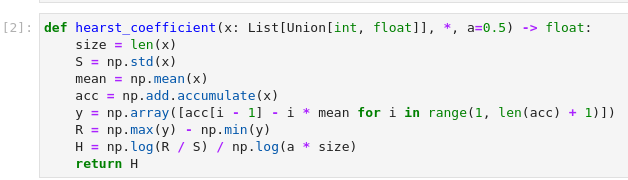
\includegraphics[scale=0.5]{hearst1}
	\caption{Функция для расчёта показателя Хёрста в Python}
	\label{fig:hearst1}
\end{figure}

Сгенерируем случайную равномерно распределённую последовательность от $[a, b]$. В качестве длины ряда возьмём значение 50, в качестве $a = 2$, а в качестве $b = 20$. (Рисунок \ref{fig:hearst2})
\begin{figure}[h]
	\centering 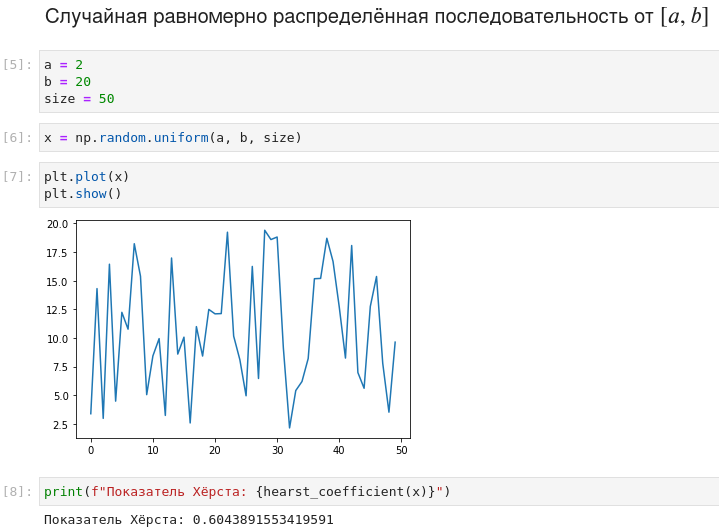
\includegraphics[scale=0.5]{hearst2}
	\caption{Расчёт показателя Хёрста для ряда, который равномерно распределён на отрезке $[a, b]$}
	\label{fig:hearst2}
\end{figure}

Показатель Хёрста в данном случае равен 0.604389, что говорит о том, что в данный ряд можно отнести к классу персистентных или трендоустойчивых -- сохраняющих имеющуюся тенденцию.\\

\newpage

Далее сгенерируем ряд, который подчиняется закону линейного тренда: $y = b + a \times t$. В качестве длины ряда возьмём значение 100, в качестве $a = 2$, а в качестве $b = 20$. (Рисунок \ref{fig:hearst3})
\begin{figure}[h]
	\centering 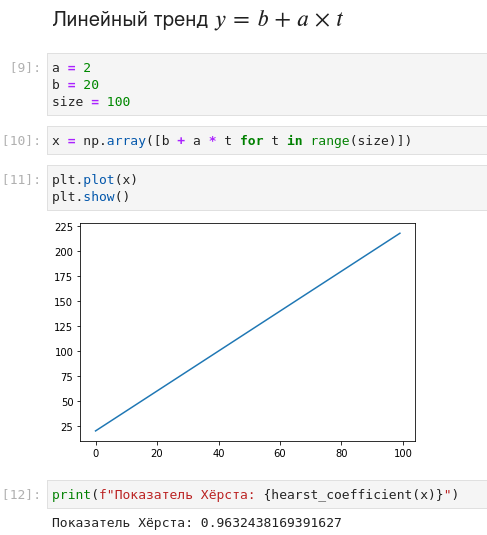
\includegraphics[scale=0.5]{hearst3}
	\caption{Расчёт показателя Хёрста для ряда, который подчиняется линейному тренду}
	\label{fig:hearst3}
\end{figure}

Показатель Хёрста в данном случае равен 0.96324, что говорит о том, что в данный ряд можно отнести к классу персистентных или трендоустойчивых -- сохраняющих имеющуюся тенденцию. Данный результат был ожидаемым для данного ряда.\\

\newpage

Далее сгенерируем ряд, который подчиняется закону линейного тренда cо случайными возмущениями: $y = b + a \times t + \epsilon$. В качестве длины ряда возьмём значение 100, в качестве $a = 2$, а в качестве $b = 20$. (Рисунок \ref{fig:hearst4})
\begin{figure}[h]
	\centering 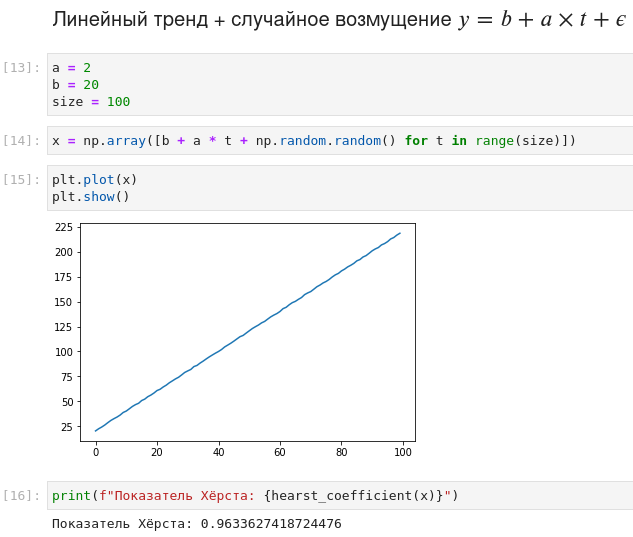
\includegraphics[scale=0.5]{hearst4}
	\caption{Расчёт показателя Хёрста для ряда, который подчиняется линейному тренду со случайными возмущениями}
	\label{fig:hearst4}
\end{figure}

Можно видеть, что на графике присутствуют некоторые возмущения, но тем не менее показатель Хёрста в данном случае равен 0.96336, что говорит о том, что в данный ряд можно отнести к классу персистентных или трендоустойчивых -- сохраняющих имеющуюся тенденцию. Данный результат был ожидаемым для данного ряда.\\

\newpage

Далее сгенерируем ряд, который подчиняется закону: $y = A \times \sin(k \cdot x)$. В качестве длины ряда возьмём значение 100, в качестве $A = 10$, а в качестве $k = 2$. (Рисунок \ref{fig:hearst5})
\begin{figure}[h]
	\centering 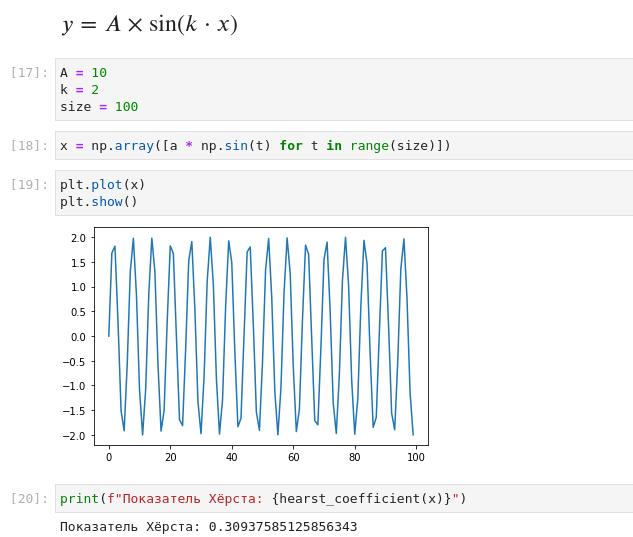
\includegraphics[scale=0.5]{hearst5}
	\caption{Расчёт показателя Хёрста для ряда, который имеет синусоидальные колебания}
	\label{fig:hearst5}
\end{figure}

Показатель Хёрста в данном случае равен 0.309375, что говорит о том, что в данный ряд можно отнести к классу антиперсистентных -- рост в прошлом означает уменьшение в будущем, а тенденция к уменьшению в прошлом делает вероятным увеличение в будущем. Данный результат был ожидаемым для данного ряда.\\

\newpage

Последний сгенерированный ряд был ряд, который подчиняется закону: $y = A \times \sin(k \cdot x)$. В качестве длины ряда возьмём значение 100, в качестве $A = 10$, а в качестве $k = 2$. (Рисунок \ref{fig:hearst6})
\begin{figure}[h]
	\centering 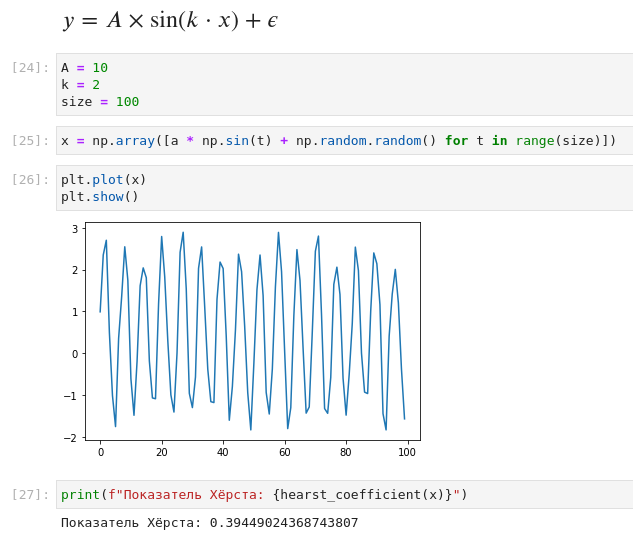
\includegraphics[scale=0.5]{hearst6}
	\caption{Расчёт показателя Хёрста для ряда, который имеет синусоидальные колебания и случайные возмушения}
	\label{fig:hearst6}
\end{figure}

Показатель Хёрста в данном случае равен 0.39449, что говорит о том, что в данный ряд можно отнести к классу антиперсистентных -- рост в прошлом означает уменьшение в будущем, а тенденция к уменьшению в прошлом делает вероятным увеличение в будущем. Данный результат был ожидаемым для данного ряда.\\

Если сравнивать его с предыдущим рядом, то значение показателя Хёрста возрасло с добавлением случайных колебаний.\\

Таким образом, были рассчитаны показатели Хёрста для различных рядов, после чего был определён класс ряда по наличию в данном ряде долговременной памяти.